%---------------------------------------------------------------------------%
%-                                                                         -%
%-                           LaTeX Template                                -%
%-                                                                         -%
%---------------------------------------------------------------------------%
%- Copyright (C) Huangrui Mo <huangrui.mo@gmail.com> 
%- This is free software: you can redistribute it and/or modify it
%- under the terms of the GNU General Public License as published by
%- the Free Software Foundation, either version 3 of the License, or
%- (at your option) any later version.
%---------------------------------------------------------------------------%
%->> Document class declaration
%---------------------------------------------------------------------------%
\documentclass[twoside,fontset=adobe]{Style/ucasthesis}%
%- Multiple optional arguments:
%- [<oneside|twoside|print>]% oneside eprint, twoside eprint, or paper print
%- [fontset=<adobe|none|...>]% specify font set instead of automatic detection
%- [scheme=plain]% thesis writing of international students
%- [draftversion]% show draft version information
%- [standard options for ctex book class: draft|paper size|font size|...]%
%---------------------------------------------------------------------------%
%->> Document settings
%---------------------------------------------------------------------------%
\usepackage[numbers,list]{Style/artratex}% document settings
%- usage: \usepackage[option1,option2,...,optionN]{artratex}
%- Multiple optional arguments:
%- [bibtex|biber]% set bibliography processor and package
%- [<numbers|super|authoryear|alpha>]% set citation and reference style
%- <numbers>: textual: Jones [1]; parenthetical: [1]
%- <super>: textual: Jones superscript [1]; parenthetical: superscript [1]
%- <authoryear>: textual: Jones (1995); parenthetical: (Jones, 1995)
%- <alpha>: textual: not available; parenthetical: [Jon95]
%- [geometry]% reconfigure page layout via geometry package
%- [lscape]% provide landscape layout environment
%- [xhf]% disable header and footer via fancyhdr package
%- [color]% provide color support via xcolor package
%- [background]% enable page background
%- [tikz]% provide complex diagrams via tikz package
%- [table]% provide complex tables via ctable package
%- [list]% provide enhanced list environments for algorithm and coding
%- [math]% enable some extra math packages
%- [xlink]% disable link colors
\usepackage{Style/artracom}% user defined commands
%---------------------------------------------------------------------------%
%->> Document inclusion
%---------------------------------------------------------------------------%
%\includeonly{Tex/Chap_1,...,Tex/Chap_N}% selected files compilation
%---------------------------------------------------------------------------%
%->> Document content
%---------------------------------------------------------------------------%
%-
%-> Titlepage information
%-
%---------------------------------------------------------------------------%
%->> Titlepage information
%---------------------------------------------------------------------------%
%-
%-> 中文封面信息
%-
\confidential{}% 密级:只有涉密论文才填写
% \schoollogo[scale=0.095]{ucas_logo}% 校徽
\title{开源RISC-V高性能处理器核分支预测部件设计}% 论文中文题目
\author{勾凌睿}% 论文作者
\advisor{包云岗~~~~中科院计算所研究员}% 指导教师:姓名 专业技术职务 工作单位
%\advisor{指导教师一\\指导教师二\\指导教师三}% 多行指导教师示例
% \degree{硕士}% 学位:学士、硕士、博士
% \degreetype{理学}% 学位类别:理学、工学、工程、医学等
\major{计算机系统结构}% 二级学科专业名称
\institute{中~~国~~科~~学~~院~~计~~算~~技~~术~~研~~究~~所}% 院系名称
%\institute{中国科学院力学研究所\\流固耦合实验室}% 多行院系名称示例
% \date{2014~年~6~月}% 毕业日期:夏季为6月、冬季为12月
\submitdate{2021.5}
%-
%-> 英文封面信息
%-
% \TITLE{aaa}% 论文英文题目
% \AUTHOR{Mo Huangrui}% 论文作者
% \ADVISOR{Supervisor: Professor Liu Qingquan}% 指导教师
\DEGREE{MasterToDoctor}% 学位:Bachelor, Master, Doctor, Postdoctor。封面据英文学位名称自动切换,需确保拼写准确
% \DEGREETYPE{Natural Science}% 学位类别:Philosophy, Natural Science, Engineering, Economics, Agriculture 等
% \MAJOR{Fluid Mechanics}% 二级学科专业名称
% \INSTITUTE{Institute of Mechanics, Chinese Academy of Sciences}% 院系名称
% \DATE{June, 2014}% 毕业日期:夏季为June、冬季为December
%---------------------------------------------------------------------------%
%
\begin{document}
%-
%-> Frontmatter: title page, abstract, content list, symbol list, preface
%-
\frontmatter% initialize the environment
%---------------------------------------------------------------------------%
%->> Frontmatter
%---------------------------------------------------------------------------%
%-
%-> 生成封面
%-
\maketitle% 生成中文封面
% \MAKETITLE% 生成英文封面
%-
%-> 作者声明
%-
% \makedeclaration% 生成声明页
%-
%-> 中文摘要
%-
\intobmk\chapter*{摘\quad 要}% 显示在书签但不显示在目录
\setcounter{page}{1}% 开始页码
\pagenumbering{Roman}% 页码符号
摩尔定律的逐渐失效使得体系结构领域进入创新的黄金年代\cite{hennessy2019new}。基于RISC-V指令集架构的开源芯片设计是有前途的发展方向,所以一款高性能的开源RISC-V处理器核实现对于工业界和学术界都意义重大。分支预测部件是保证处理器指令供给的重要结构,现有的开源分支预测部件都没有同时达到高预测性能和高主频的要求。本文的工作实现了香山开源RISC-V高性能处理器核中的分支预测部件。它采用三级覆盖预测结构,在已有开源设计的基础上,实现了最大分支历史长度为64的TAGE-SC-L分支方向预测器\cite{seznec2014tage};全局分支历史采用了一种新机制管理,避免了多级预测下因不同流水级分支历史不同而造成的自身冲刷;跳转目标地址采用256项MicroBTB和2048项BTB预测;返回地址的预测使用16项RAS。本实现在TSMC~28nm工艺下评估达到1.5GHz主频。

\keywords{RISC-V,开源芯片设计,分支预测部件设计,全局分支历史}% 中文关键词
%-
%-> 英文摘要
%-
\intobmk\chapter*{Abstract}% 显示在书签但不显示在目录
With the foreseeable end of Moore's Law, there comes a gloden age of innovation for computer architecture\cite{hennessy2019new}. Open-source chip design on RISC-V ISA is expected to have a promising future, so the implementation of an open-source high-performance RISC-V core is of great significance to the industry and academia. Branch prediction unit is an important structor to ensure sufficient supply of instruction to the execution core. None of the existing open-source branch prediction unit implementation meet the requirements of high prediction accuracy and high frequency at the same time. We implemented the branch prediction unit in XiangShan open-source RISC-V high performance processor, which adopted a three-level overriding structure. On the basis of existing open-source design, we implemented a TAGE-SC-L branch predictor\cite{seznec2014tage} with maximum history length of 64. We introduced a new method of global history management, preventing self flushes due to the inconsistency of global history value among different pipeline stages in an overriding structure. We used a 256-entry MicroBTB and a 2048-entry BTB to predict the target of control flow instructions, with a 16-entry RAS for retrun address prediction. This implementation achieved 1.5GHz under TSMC~28nm process. 

\KEYWORDS{RISC-V, Open Source Chip Design, Branch Predictor Component Design, Global Branch History}% 英文关键词
%---------------------------------------------------------------------------%% title page, abstract
{% content list region
\linespread{1.2}% local line space
\intobmk*{\cleardoublepage}{\contentsname}% add link to bookmark
\tableofcontents% content catalog
\intobmk*{\cleardoublepage}{\listfigurename}% add link to bookmark
\listoffigures% figure catalog
\intobmk*{\cleardoublepage}{\listtablename}% add link to bookmark
\listoftables% table catalog
}
% \input{Tex/Prematter}% symbol list, preface content
%-
%-> Mainmatter
%-
\mainmatter% initialize the environment
%---------------------------------------------------------------------------%
%->> Main content
%---------------------------------------------------------------------------%
\chapter{引言}\label{chap:intro}

\section{研究背景}

随着芯片制程的提高,现有工艺逐渐逼近物理极限,摩尔定律和丹纳德缩放比例定律走向终结。Patterson和Hennessy在图灵演讲中指出,体系结构领域正走向变革的黄金时代\cite{hennessy2019new},人们不再能仅依靠制程的进步逐年在芯片上实现更复杂的架构。他们认为领域专用架构是接下来芯片性能提升的重点。然而,随着制程进步,芯片复杂度变高,从而导致芯片的设计成本不断攀升,这阻碍了创新性的想法和设计付诸实践。

针对这个问题,软件行业已经有了开源作为答案。开源的意义在于成果共享,避免重复劳动,提升行业整体效率。以Linux为核心的开源软件栈,大大减少了开发者去开发一款新应用的时间和人力投入,有了诸如GCC之类的开源实现,用户只需要复用这些软件和库,需要自己实现的逻辑大大减少。同时开源和商业也并不冲突,选择适当的开源协议,可以让开源的成果为商业所用。RedHat就是Linux商业化的最著名的例子。

受到软件行业的启发,硬件行业也引入了开源的概念,首先诞生了一款设计理念先进并且开放授权的指令集设计RISC-V\cite{asanovic2014instruction}。它自从诞生以来在工业界和学术界的影响力与日俱增。在此基础上,一款成功的、高性能的RISC-V处理器核实现,不论对于工业界还是学术界都至关重要。这样的实现可以降低工业界IP的授权成本和开发周期;而学术界可以将其作为一个比软件模拟器更精准的体系结构探索平台。理想情况下,它可能成为开源芯片领域类似Linux的存在。而一些新的硬件构造语言例如Chisel\cite{bachrach2012chisel}、SpinalHDL等,将编程语言的高级特性与硬件设计相结合,进一步提高了硬件代码的表达能力,从而提升了芯片敏捷开发的可能性。

\section{研究动机}
\subsection{现有分支预测部件设计的不足}
尽管目前有一些开源的分支预测部件设计,但它们都没有同时做到高预测和高主频。分支方向预测器对于分支预测部件至关重要,目前state-of-the-art级别的分支方向预测器主要有两种:TAGE\cite{seznec2006case}和perceptron\cite{jimenez2001dynamic}。当前开源高性能处理器核的实现中,在分支预测器部分实现了两者之一的只有加州伯克利的SonicBOOM\cite{zhao2020sonicboom},但它并没有经过流片验证。经我们评估,其主频只能达到不到1GHz。因此,目前并没有符合要求的高性能分支预测部件设计。

\subsection{分支预测部件设计的挑战}
针对现有开源分支预测部件设计的补足,本工作旨在实现同时达到高预测性能和高主频的分支预测部件。

对于预测性能方面,主要有如下的评价指标:预测宽度、分支时延和预测准确率。下面将会对它们进行逐点的分析:
\begin{itemize}
    \item 预测宽度需要配合取指宽度,取指宽度又与后端流水线宽度息息相关,前端的取指宽度需要保证后端的指令供给;
    \item 现代处理器主频逐渐提高,与此同时分支预测策略也渐趋复杂,导致难以在愈发有限的时钟周期内完成复杂的分支预测任务\cite{jimenez2000impact}。工艺制程上的进步并不能解决两者的冲突,以TAGE分支方向预测器\cite{seznec2006case}为例,它的预测流程至少要分为历史折叠、存储表访问和选择最长匹配三个阶段,这三个阶段都需要一个时钟周期完成。在很宽的取指宽度下,大概率每一拍都会遇到分支指令。如果每一条分支指令都要等到数个时钟周期后出结果,那么最终的指令供给将无法达到处理器后端的要求;
    \item 前两个指标保证了前端能给后端足够的指令供给,而预测准确率保证了这些指令供给的有效性。如果误预测率很高,前端取到的很多指令都在错误的执行路径上,最终会被冲刷掉。即使供指带宽很高,处理器得到的真实指令供给也会不足,导致整体性能不高。
\end{itemize}

在预测性能一定的前提下,整体性能和频率成正比,高主频对于总体性能至关重要。本设计的基本目标是让分支预测部件的主频达到1.5GHz,避免成为整个处理器核的频率瓶颈。

\section{论文的主要内容与贡献}
针对前述指标和挑战,本工作在参考已有实现的基础上,在香山开源RISC-V处理器核中实现了一款高性能分支预测部件,初步解决了这些问题。

我们采用全并行的预测方法实现高预测宽度,达到了最大16条指令/周期的预测宽度;用覆盖预测架构解决主预测器长分支时延的问题,实现了最佳情况下无空泡的取指;通过优化主预测器的误预测率,降低分支预测部件的整体误预测率,在SPEC CPU 2006\cite{henning2006spec}上达到了4.17的MPKI;最后,通过一系列细节上的优化,使频率达到了1.5GHz。

\section{论文组织}
本文的后续章节组织结构如下:

第\ref{chap:design}章介绍了香山处理器分支预测部件的设计,包括其整体预测架构、一些子预测部件的设计以及在此架构设计下的预测流程。

第\ref{chap:impl}章介绍了香山处理器分支预测部件的实现,包括本工作的代码基础和所选用的语言,也介绍了实现上一些关键问题的处理方案,包括分支历史的管理、跨取指包的RVI指令的预测以及预测器更新的问题。

第\ref{chap:eval}章介绍了香山处理器分支预测部件的验证和评估工作,其中评估部分包括后端评估和预测性能评估。

第\ref{chap:result}章对本文工作进行总结,并提出了接下来可能的研究方向。
% \input{Tex/Chap_Guide}
% \chapter{背景}\label{chap:background}

\chapter{分支预测部件微架构设计}\label{chap:design}
本章我们详细介绍香山处理器核分支预测部件的微架构设计。首先我们对于前述影响性能的各项指标,描述我们针对性的设计思路。接着详细介绍分支预测部件中的模块及每个模块的功能。

分支预测部件和取指部件关联紧密,它们之间的关系主要有两类:
\begin{enumerate}
    \item 紧耦合:取指和预测流水完全同步;
    \item 解耦\cite{reinman1999scalable}:先预测后取指,用队列连接。
\end{enumerate}

出于项目进度的考虑,我们选择紧耦合实现。
\begin{figure}[!htbp]
    \centering
    \includegraphics[width=\textwidth]{bpu}
    \caption{分支预测部件结构示意图}
    \label{fig:bpu}
\end{figure}
\section{设计思路}
图\ref{fig:bpu}展示了分支预测部件的结构。我们首先用一个小节阐述我们在前述关键指标驱动下的设计思路。
\subsection{并行预测以提高预测宽度}
香山处理器核的后端是六发射结构,理想情况下每拍能消耗前端取指单元提供的六条指令。为了满足后端的指令供给,取指宽度至少不小于六。我们为了留出一些余量,将取指宽度设置为32字节,以标准RVI指令计算,每拍最多取出八条指令。由于香山处理器核实现了RISC-V压缩指令扩展,指令大小可能为二或四字节,所以每拍实际上能取出最多十六条指令(假如全部是压缩指令)。在这样的取指宽度下,每一次取指遇到一条甚至多条转移指令的概率很大,因此我们需要支持多条指令的并行预测以避免行内指令的结构相关带来的性能损失。香山处理器核分支预测部件采用了全并行预测的设计,对于一次取到的32字节中的全部16个可能的指令起始位置都进行预测。
\subsection{流水化覆盖多级预测以降低分支时延}
我们实现的主分支方向预测器的访问延迟是三个时钟周期,为了缓解分支时延,我们首先将各分支预测部件流水化,让它们在流水线后端不阻塞的情况下,每一周期都能处理一个新的取指请求。如果仅是这样,对于一条分支指令,它仍需要三个时钟周期才能得到预测结果,而与其相邻的下一个取指请求依赖于这条分支指令的预测结果。为了达到不阻塞流水线的目的,简单的处理办法是在分支预测结果尚未得到时,默认其不跳转。于是对于实际执行结果不跳转的分支指令,相当于没有流水线空泡。但对于实际跳转的分支指令,则需要在得到预测器结果时,向之前的流水级发送重定向请求,执行流水线冲刷,这样仍存在流水线的空泡。为了解决这个问题,我们在设计上引入多级覆盖预测,额外使用一些时延较小的简单的分支预测部件,很快地得到一个准确率相对较低的预测结果,用于快速发出下一个取指请求。当主预测器的预测结果与简单预测器不符时,再冲刷流水线,并根据主预测器的预测结果重新发出取指请求。这样能够进一步将跳转分支的预测时延限制在简单预测器和主预测器结果不符的情况下。
\subsection{使用TAGE-SC-L提高分支方向预测准确率}
% 程序依赖分支指令构成控制流,现代程序平均每五条就有一条分支指令,因此分支指令的准确预测对处理器总体性能至关重要。分支指令的执行有两个基本要素:跳转方向和目标地址,分支预测需要同时解决这两个问题。对于RISC-V指令集架构来说,条件分支属于直接跳转,其目标地址由指令地址加上指令码中指定的偏移计算,因此一般情况下是不会改变的,比较容易预测。而条件分支的跳转方向会随程序行为变化而变化,属于分支预测的重点。目前业界普遍的做法是全局分支历史信息在逻辑上可以用一个移位寄存器实现,顺序记录了到当前周期为止,执行过的前n条分支指令的跳转方向。每当一条分支指令被执行,便在移位寄存器中移入一位,并移出最老的一条分支的信息。
为了提高分支方向预测准确率,我们引入了TAGE-SC-L预测器\cite{seznec2014tage}作为分支方向的主预测器。TAGE-SC-L是目前学术界state-of-the-art的分支预测方法。它主要利用长度呈几何级数的全局分支历史信息经异或折叠后与程序计数器PC的值哈希,分别用于索引多个表中的项,并对于每个表计算一个Tag,用于判断是否匹配,其预测结果由匹配到的使用最长历史长度的那个表决定。TAGE-SC-L的具体算法较为复杂,此处不再赘述。

\section{分支预测架构}
本节详细介绍分支预测部件的架构。如图\ref{fig:bpu}所示,分支预测部件主要由各子预测部件和顶层逻辑组成,另外还包括实现于取指部件中的分支历史管理逻辑。

各子预测部件包括:
\begin{itemize}
    \item MicroBTB(uBTB):分支目标微缓冲,提供一周期内的分支方向和跳转目标预测;
    \item BTB:分支目标微缓冲,提供两周期内的跳转目标地址预测;
    \item BIM:作为BTB的补充,在两周期内用两位饱和计数器提供分支方向预测;
    \item TAGE-SC-L:主分支方向预测器,在三周期内提供分支方向的准确预测;
    \item RAS:返回地址栈,在最后一周期为返回指令提供目标地址预测。
\end{itemize}

顶层逻辑主要将各子预测部件的预测按流水级以统一的接口输出供取指模块使用,以及处理部分子预测部件的结果需要在多个流水级复用的情况。虽然分支预测部件整体是流水化的,但由于它和取指单元紧耦合,因此它只需要复用取指单元的握手信号,便可以驱动自身流水级的行进。

接下来将沿一个取指请求的预测流程,详细介绍几个子模块及其处理逻辑。每一级都会对每一条指令是否跳转,以及其在跳转情况下的目标地址进行预测。

\subsection{第一级预测:MicroBTB}
取指请求PC暂存一拍后,送入MicroBTB进行访问,从MicroBTB的全相联CAM中,根据PC高位生成的Tag判断每一条指令是否命中。如果不命中则视为不跳转(不论是否是转移指令);如果命中则根据其中存储的isBr状态位,决定是否使用对应的两位饱和计数器的结果判断条件分支方向。若isBr为1,则该指令是条件分支,用两位饱和计数器的高位作为预测的方向;反之则是无条件跳转,默认跳转。

\subsection{第二级预测:BTB和BIM}
取指请求PC经过存储映射逻辑,直接输入BTB和BIM的SRAM的读端口,在下一个时钟周期得到预测信息。对于BTB的预测信息,和MicroBTB的处理类似,根据Tag判断每一条指令的命中情况,并根据命中情况决定是否使用BIM的分支方向预测信息。这些逻辑做完后暂存一拍,在第二个流水级使用预测结果。

\subsection{第三级预测:TAGE-SC-L和RAS和预译码信息}
与取指请求对应的分支历史在暂存一拍后,根据不同表的历史长度和表项个数进行异或折叠,折叠后与暂存一拍的取指请求PC哈希后分别得到访问SRAM的索引和用于匹配的Tag。索引直接送入TAGE-SC-L的SRAM的读端口,而Tag暂存一拍,与下一个时钟周期得到的预测数据结合,经过Tag匹配和最长历史选择等逻辑后得到最终的分支方向预测,暂存一拍后用于第三级流水的分支方向预测。

RAS是一个栈结构,它的预测永远来自栈顶项,只需要在第三级流水根据预译码给出的转移指令类型信息,决定是否让某一条指令的目标地址预测选择来自RAS的结果。

预译码信息来自取指模块,根据指令Cache取出的指令码进行简单的译码操作,结果在第三个流水级送入分支预测部件使用。它提供转移指令的类型信息,以及条件分支和无条件直接跳转类型指令的目标地址。

\section{预测器的恢复和更新}\label{design:restore_update}
各个子预测部件在预测时都会产生一些预测相关的信息,它们需要被保存下来,以待将来的误预测恢复和提交后更新。当产生分支误预测,前端收到重定向请求时,有一些预测器的状态经历了推测更新,已经和错误分支刚刚预测结束时有所差别,这时候就需要用保存下的信息将预测器状态恢复到预测完目标分支之后的状态,从而保证正确路径上的分支所用的分支历史等信息都是正确的。当转移指令提交时,相应的预测信息会送回各子预测部件进行相应的表项更新。香山处理器中的预测信息存储放在了一个独立的队列中实现。当最后一级预测完成时,会将该取指请求对应的所有指令的预测信息作为一项入队;在该取指请求取到的所有指令都提交完成后,该项出队。
\chapter{分支预测部件实现}\label{chap:impl}
本章我们详细介绍香山处理器核分支预测部件的实现。我们首先介绍我们选用的硬件描述语言以及代码基础;接着详细介绍一些关键问题的处理方案。

\section{语言和代码基础}
我们的工作基于加州伯克利大学开源的BOOM(Berkeley Out of Order Machine)\cite{asanovic2015berkeley}。它的第三代SonicBOOM\cite{zhao2020sonicboom}是目前性能最高的RISC-V开源乱序处理器核。它的主分支预测器是L-TAGE\cite{seznec2011new},同样实现了三级覆盖预测结构,但它的频率经评估后只能达到800MHz。

我们在借鉴其总体架构的基础上,复用了其中的部分模块,对一些细节点进行优化,并为L-TAGE\cite{seznec2011new}添加了Statiscal Corrector,实现了TAGE-SC-L\cite{seznec2014tage}分支方向预测器。此外,我们还优化了它的时序,极大地提升了频率。

我们选用了Chisel硬件构造语言\cite{bachrach2012chisel}。它由加州伯克利大学在Scala编程语言的基础上进行开发,实现了一种可以结合高级语言的面向对象和函数式特性的,可以设计高度参数化硬件的语言。它提高了硬件设计的抽象水平,极大地提高了开发效率和可维护性。

\section{关键问题的处理方案}
\subsection{分支历史的管理}
现代分支预测器依赖处理器执行过程中记录的全局分支历史信息,在取指单元进行基于硬件的动态预测,因此分支历史的管理是分支预测部件中至关重要的部分,而准确的分支历史则是高预测准确率的保障。在分支预测部件的实现中,在分支历史的管理方面主要遇到了两个问题:
\begin{enumerate}
    \item 分支历史中的一位表示什么含义?\label{his:q1}
    \item 如何处理多级预测过程中产生不同的分支历史的情况?\label{his:q2}
\end{enumerate}

\subsubsection*{问题\ref{his:q1}}
分支历史的普遍含义是,到当前周期为止,执行过的前n条分支指令的跳转方向。这个含义下,一位分支历史表示某一条动态分支指令的跳转方向。在所有指令全并行预测的框架下,一个时钟周期可能同时预测多条分支指令,如果要对每一条分支指令都计算分支历史,那么会产生17种可能的移位结果,分别对应行内存在0\textasciitilde16条分支指令的情况;而对每一种移位结果中的其中一位新历史而言,它的值也有16种可能的来源。以上两者对应到逻辑上分别是一个17-1和16-1多路选择器,且两者是串行逻辑。如果用二叉树实现,它们最终分别会引入5级和4级逻辑门,两者之和是9级逻辑门。而分支历史的推测更新是时序关键路径所在,此路径上的9级逻辑门是不可接受的。我们为了降低实现复杂度,采用了和BOOM相同的做法,将整个取指请求的所有分支历史压缩成一位,每一拍最多更新一位分支历史。这样是否更新分支历史只取决于行内是否存在有效的分支指令,而更新结果取决于行内有效的分支指令中是否有跳转的。有效分支指令的含义是,该指令位于行内取指PC之后的位置,且在它前面没有跳转的转移指令。由于一行最多只有一条跳转的转移指令,所以行内存在有效跳转分支指令的等价条件是:行内第一条跳转的指令是分支指令。如上的机制减少了分支历史的逻辑复杂度。同时,由于一个取指请求内可能存在多条分支指令,在相同长度的分支历史寄存器配置下,等效的分支历史长度变长了。

\subsubsection*{问题\ref{his:q2}}
为了得到准确的分支历史信息,必须在预测的同时用预测结果对历史进行推测更新,同时也必须在误预测时进行历史状态的恢复。在多级预测的语境下,最新的分支历史信息必须在第一级预测开始时得到。但在第一级预测开始时,它的上一个预测的最终结果还没有拿到。在这种情况下,即使最终的预测结果是正确的,但其相邻的下一个预测所用的分支历史可能是不准确的。由于最终预测结果是正确的,所以后端执行单元也不会检测到预测错误,也就不会发出重定向请求。使用了错误分支历史信息的指令会存在于正确路径上,这与\ref{design:restore_update}中的假设相悖,会导致最终预测性能的损失。

针对这个问题,SonicBOOM\cite{zhao2020sonicboom}实现了简单的解决方案。它在每一级预测结束后检查结果是否与之前的预测相符时,也对预测后推测更新的分支历史进行检查,如果存在不一致,则也冲刷该级之前的流水线。这种方案可以保证正确路径上的预测所用的分支历史也都是正确的,但可能会增加许多预测流水线自冲刷,从而增加取指空泡。

我们在实现中采用了另一种方案。将分支历史寄存器维护在最后一级预测结束后,在最后一级预测结果成功进入下一级流水时更新分支历史寄存器。为了在第一级预测之前获取到最新的分支历史,我们在每一拍都对全部的三个预测结果进行检测,同时按照取指顺序的先后,根据当前所见的预测结果,用正常的历史更新逻辑倒推出最新的分支历史。\\
如图所示\\
在预测结束后,将开始预测时所用的分支历史,和预测结束前看到的分支历史寄存器中的历史(它们可能不同)同时存进分支预测信息的队列。在误预测恢复的时候,将分支历史寄存器重置为预测结束时所见该寄存器中的内容,并根据真实预测结果进行更新;而当预测器表项在分支指令提交更新的时候,以预测时所见的分支历史为准进行更新操作。这样,对于分支历史寄存器,正确路径上的分支指令见到的仍然是准确的分支历史。而对于预测时所使用的分支历史,它的值取决于该条指令的前三个取指请求在预测流水线上的分布和预测结果。只要这两者在相同情况下能保持一定的稳定性,那么最终的预测性能将不会有大的损失。

在这种机制下,前端自身不会产生因分支历史不同而导致的取指空泡,可能的代价包括:
\begin{enumerate}
    \item 多存一份用于更新的分支历史所带来的存储开销
    \item 预测历史不完全准确带来的性能损失
\end{enumerate}
只要此方法的存储开销在可接受的范围内,而预测准确率的损失能被减少的取值空泡掩盖,此方法便有可行性。我们的初步评估结果显示,此方法相对另一种还有性能提升。

\subsection{跨取指包的RVI指令的预测}
由于分支预测和取指紧耦合,分支预测部件实际上需要对取指取到的所有有效指令做预测。出于实现复杂度和时序方面的考虑,我们以取指宽度(32字节)对齐的地址向指令缓存发出取指请求,得到的指令码会根据取指的实际起始PC进行舍弃,仅保留实际起始PC之后的部分。由于带压缩扩展的RISC-V指令集存在两种指令长度:2字节和4字节,实际指令的放置是按2字节对齐的。在上述机制下,会出现一条4字节长的指令被32字节对齐的地址分为两段的情况。此种情况下,第一个取指请求不会认为此指令有效,因为当时并未得到完整的指令。而按照正常的逻辑,指令的预测依据的是指令的开端所在的PC。当一条4字节长的转移指令被32字节对齐的地址分成两段,如果不经特殊处理,就会出现如下情况:它的预测信息在前一个32字节的预测中被读出并丢弃。原因是:在没有拿到完整的指令的前提下,即使预测部件认为它是一条转移指令并预测跳转,也不能直接从跳转目标地址开始下一次取指。这是由于此类指令在我们目前取指逻辑和预测逻辑中的位置有所偏差导致的。如前所述,在预测逻辑中,指令位于指令开端所在的PC。而在取指逻辑中,对于这类指令会记录下它的前半段指令码,待下半段指令码所在的32字节被取回后,将其与对应的后半段指令码拼起来,作为该取指请求中取到的第一条指令。因此,一条这样的RVI指令,在取指单元中的实际指令位置,处于它的后半段指令所在PC。

如果要正确地预测上述情况的转移指令,必须通过某种形式将它的预测信息和在实际取指逻辑中所处的位置结合起来。一种最直接的想法是在这种情况下把预测信息像前半条指令的指令码一样寄存起来,等到预测后半条指令时再插入。这种方法增加了一些寄存器开销,也在预测关键路径添加了一部分逻辑。我们采用了另一种方法,使得这类指令的预测信息自然地写入到后半条指令所对应的位置。我们利用了存储预测信息的队列以取指请求为单位的特性,让预测信息的更新也以取指请求为单位发出。这样一来,前述的位置偏差就不存在了。对于跨取指请求的RVI转移指令,它的更新请求随着它被取到的那个取指请求发出,也就是它的后半段指令所在的位置。而对于其余的转移指令,仍旧更新到了指令开端PC所在的位置。


\subsection{预测器更新问题}
理想的分支预测器假设预测后根据执行结果和表项的预测时状态(即当前状态)即刻更新,但在真实的实现中这两者都不能满足。真实处理器实现有着如下的特点:
\begin{enumerate}
    \item 预测后不可能马上得到真实执行结果,且往往为了保证预测内所含信息的准确性,会在分支指令真正提交时才进行更新,以防止错误路径上的分支污染预测器表项,这样预测和更新就会存在时间差;
    \item 假如用SRAM实现预测器存储,如果要在更新时得到当前状态,需要对SRAM再进行一次读操作,而多口SRAM存储效率相比单口SRAM差距很大,反之若与预测读请求竞争读口,对预测流水线效率影响很大,通常会将预测时的状态暂存下来等到更新时使用;
\end{enumerate}

需要指出的是,在如上的条件下,预测时读出的状态可能是没有经过妥善地更新的。这是因为在一条指令预测的时间点,在处理器的流水线中还存在尚未提交更新的分支指令,其中可能恰好存在同一条静态分支。在更新时,我们无法区别误预测的原因究竟是不是由于预测时使用了“旧”的表项信息。在我们的具体实现中,我们参考BOOM的做法,采取了一种妥协性的做法。我们实现了一个写入前缓存逻辑,在写入SRAM的同时也将写入的索引和内容记录下来。当一个新的更新请求来到时,我们根据暂存的预测信息和执行结果决定写入表项的位置。同时查询写入前缓存,如果存在相同索引的缓存,就以其中的内容代替暂存的预测时状态,在它的基础上得到表项更新后的内容;如果不命中,则仍旧以暂存的预测状态为基础进行更新。这样对于频繁执行的分支,它会保持在写入缓存内,也就会一直在最新状态的基础上进行更新。写入前缓存是寄存器全相联实现,它部分模拟了预测前读表项的操作,对预测和更新时间差带来的性能损失有所弥补。

% \chapter{时序优化}\label{chap:timing}
作为一项以流片为目标的微架构设计,频率指标是决定最终性能的关键一环,因此时序达标是一项硬性要求。这项设计最初通过仿真时,频率经评估只能达到800MHz。经过与后端团队配合为期数月的时序迭代优化后,最终的频率在TSMC~28nm下达到了1.5GHz。时序调优的过程充斥着大量的工程细节,本章首先总结时序调优的基本原则和方法,接着描述我们在调优过程中的一些典型例子。
\chapter{验证和评估}\label{chap:eval}
本章主要介绍分支预测部件的验证和评估工作。验证部分包括分支预测部件的功能规格和需要验证的方面,验证工作的难点以及验证方案;评估部分主要包括后端评估和性能评估。
\section{验证}
对香山处理器核分支预测部件的验证主要包括两个方面:正确性验证和性能验证。对于分支预测部件来说,它的预测正确与否不应该影响处理器执行的正确性,因此不能通过处理器的整体功能正确与否来验证分支预测部件的正确性,它对处理器核的一切影响都应该局限在性能方面。出于整体项目的时效性考虑,我们用性能验证涵盖了正确性验证。


\section{评估}
\subsection{后端评估}
\begin{figure}[!htbp]
    \centering
    \includegraphics[width=0.8\textwidth]{gds}
    \caption{前端取指模块版图}
    \label{fig:gds}
\end{figure}
我们使用后端工具进行综合以及布局布线,在TSMC 28nm工艺下对香山处理器分支预测部件进行了评估。由于分支预测部件和取指部件紧耦合,所以将前端供指模块作为一个整体进行评估,最后生成的版图如图\ref{fig:gds}。其中蓝色矩形方框内是TAGE-SC-L预测器\cite{seznec2014tage}的SRAM,黄色矩形方框内是BTB的SRAM,这两者占了分支预测部件存储开销的绝大多数。其余如RAS之类的寄存器实现的子部件,在此处和组合逻辑一样并未标出。红色方框内是取指模块IFU的顶层逻辑,白色方框内是指令缓存的SRAM。我们进行评估的配置如表\ref{tab:config}:
\begin{table}[!htbp]
    \centering
    \footnotesize% fontsize
    \setlength{\tabcolsep}{4pt}% column separation
    % \renewcommand{\arraystretch}{1.2}%row space 
    \begin{tabular}{|c|p{5cm}<{\centering}|}
        %\cline{2-9}% partial hline from column i to column j
        \hline
        取指宽度 & $32$Bytes \\
        \hline
        MicroBTB & 共$256$项,16路全相联 \\
        \hline
        BTB & 共$2048$项,2路组相联 \\
        \hline
        BIM & 共$4096$项 \\
        \hline
        \multirow{2}*{TAGE} & 历史长度:$64$ \\
        \cline{2-2}
        & 历史表数目:$6$\\
        \hline
        \multirow{2}*{SC} & 历史长度:$32$ \\
        \cline{2-2}
        & 历史表数目:$5$\\
        \hline
        Loop~Predictor & $256$项 \\
        \hline
        RAS & $16$项 \\
        \hline
    \end{tabular}
    \caption{香山处理器分支预测部件配置列表}
    \label{tab:config}
\end{table}
\subsubsection*{时序及关键路径}
经评估,如上配置的香山处理器核分支预测部件,频率可达1.5GHz,其中的关键路径是:从TAGE-SC-L的SRAM读出预测数据,经多级预测逻辑最终反馈到SRAM的读地址的路径。这条路径跨越多个流水级,从SRAM读出开始,经过TAGE-SC-L的预测逻辑,到产生最后一级预测结果,通过覆盖预测逻辑生成SRAM的读地址。这条路径上的逻辑都是前端预测的必要逻辑,可能的解决方案包括以下几种:
\begin{enumerate}
    \item 降低TAGE-SC-L的表项个数,缩小SRAM规模,减小面积,降低读延迟;
    \item 降低TAGE-SC-L的历史表个数,减小面积,减少最长历史命中选择逻辑;
    \item 增加流水级。
\end{enumerate}
以上的方案或降低预测准确率,或增加前端取指空泡,对整体性能都有负面影响。如果不更改整体架构,需要结合处理器核整体情况,决定是否通过降低IPC来提高频率。
\subsection{性能评估}
\subsubsection{评估环境介绍}
本工作结合仿真器和模拟器对分支预测部件的RTL代码进行性能评估。仿真工具使用了周期精确的Verilator 4.201,模拟器使用了Gem5,它同样可以周期精确地对处理器架构进行模拟。为了对分支预测部件的RTL进行测试,我们使用Verilator对香山处理器核进行全核仿真,并收集运行结束打印出的性能计数器数据。为了验证RTL代码的性能,我们使用Gem5模拟器中的O3乱序处理器核实现与香山分支预测部件的主预测器进行对齐,并运行同样的测试,通过性能计数器收集数据进行对比。主要的评价指标是MPKI,即每千条指令的误预测条数,它可以反应处理器运行过程中分支预测的整体性能。

\subsubsection{测试程序介绍}
为了全面测试分支预测部件的性能,我们选用了SPEC CPU 2006\cite{henning2006spec}中的部分子项进行测试。出于时间和仿真器运行时间的限制,我们使用SimPoint方法对各项测试程序进行采样,通过运行其中的多个片段进行加权,得到某项测试最终的总体性能。我们对各个测试点用它之前的50M指令片段进行预热,使处理器核运行到采样点时,它的内部各项状态基本符合实际运行时的情况。最终计入性能统计的片段长度同样是50M。

\subsubsection*{主预测器总体预测性能}
\begin{figure}[!htbp]
    \centering
    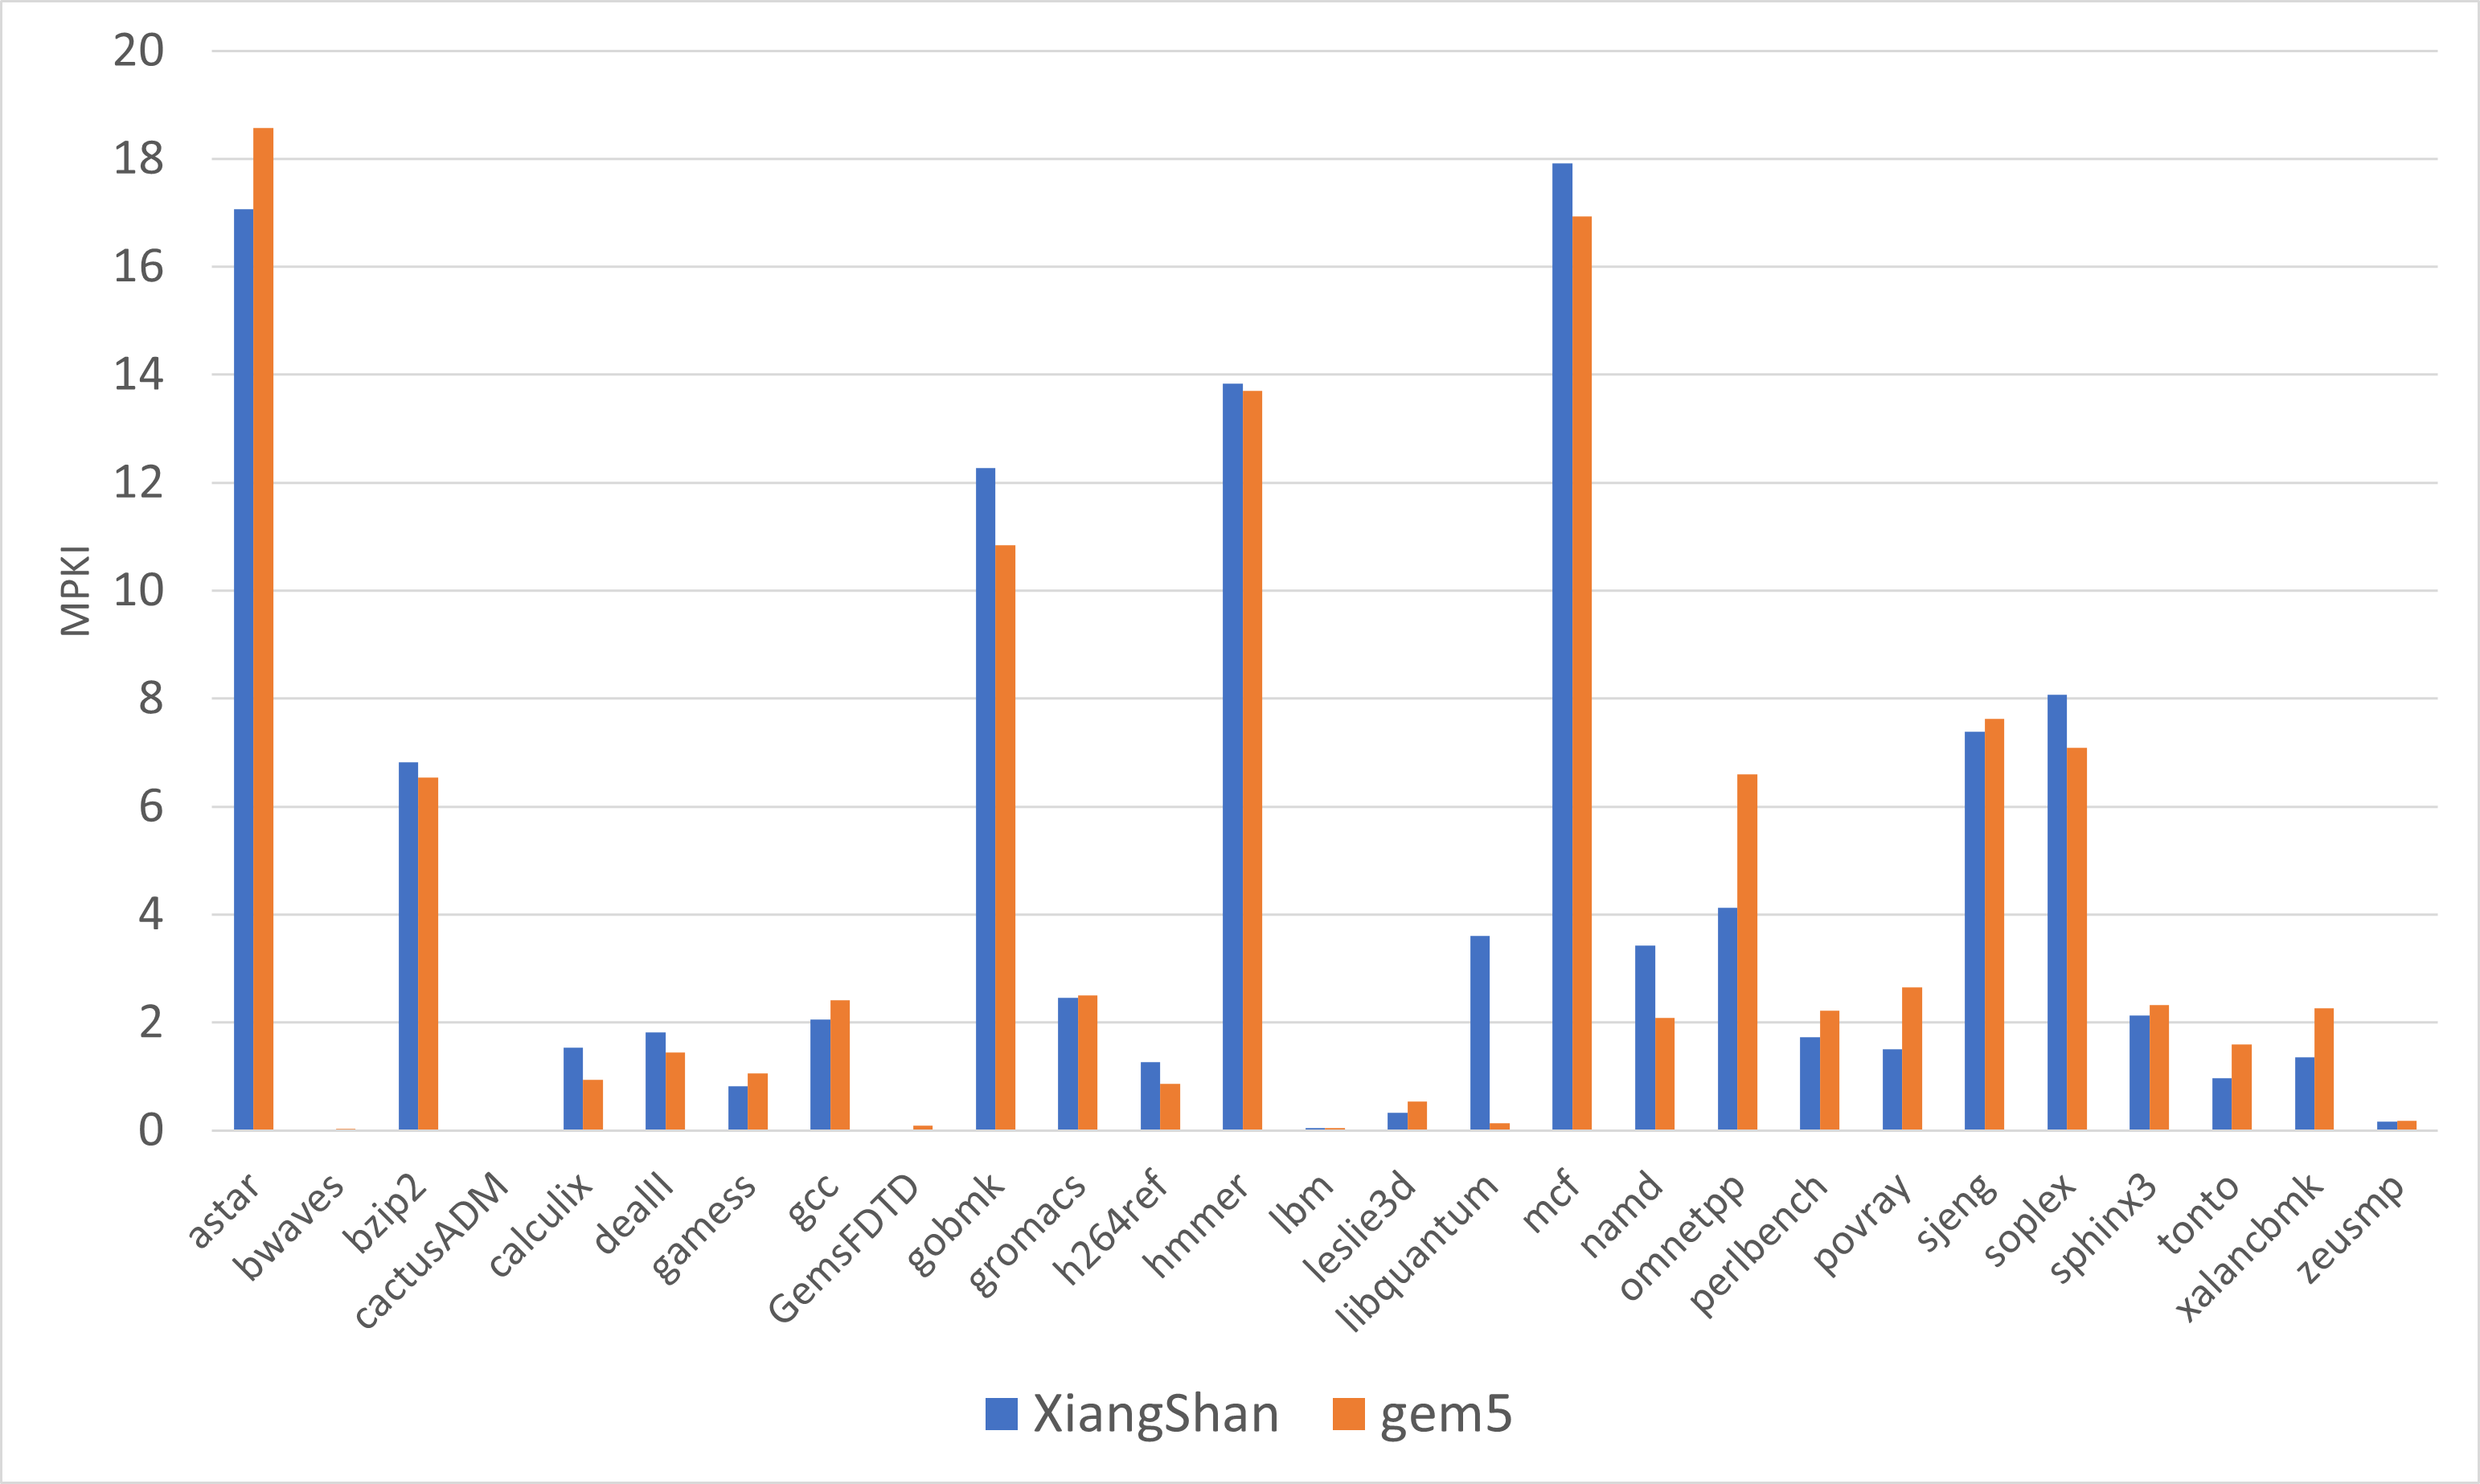
\includegraphics[width=0.9\textwidth]{xs-gem5-mpki}
    \caption{同配置下香山分支方向预测和Gem5分支预测MPKI对比}
    \label{fig:xs-gem5-mpki}
\end{figure}
主预测器决定了分支指令最终的预测结果,其误预测率是分支预测部件总体性能的关键一环。出于项目进度的考虑,我们并未对其进行形式化验证,而是在Gem5实现相同规格和算法的条件分支方向预测器,并将两者运行相同测试集的误预测率进行对比。得到的结果如图\ref{fig:xs-gem5-mpki}所示。可以看到两者在大部分测试集上预测性能近似,在个别测试集例如libquantum上预测性能差距相对较大。在所选取的测试集上,香山处理器分支预测部件主预测器的平均MPKI是4.17,同等配置下Gem5的平均MPKI是4.12。

\subsubsection*{Statistical Corrector实现效果}
\begin{figure}[!htbp]
    \begin{subfigure}{.45\textwidth}
        \centering
        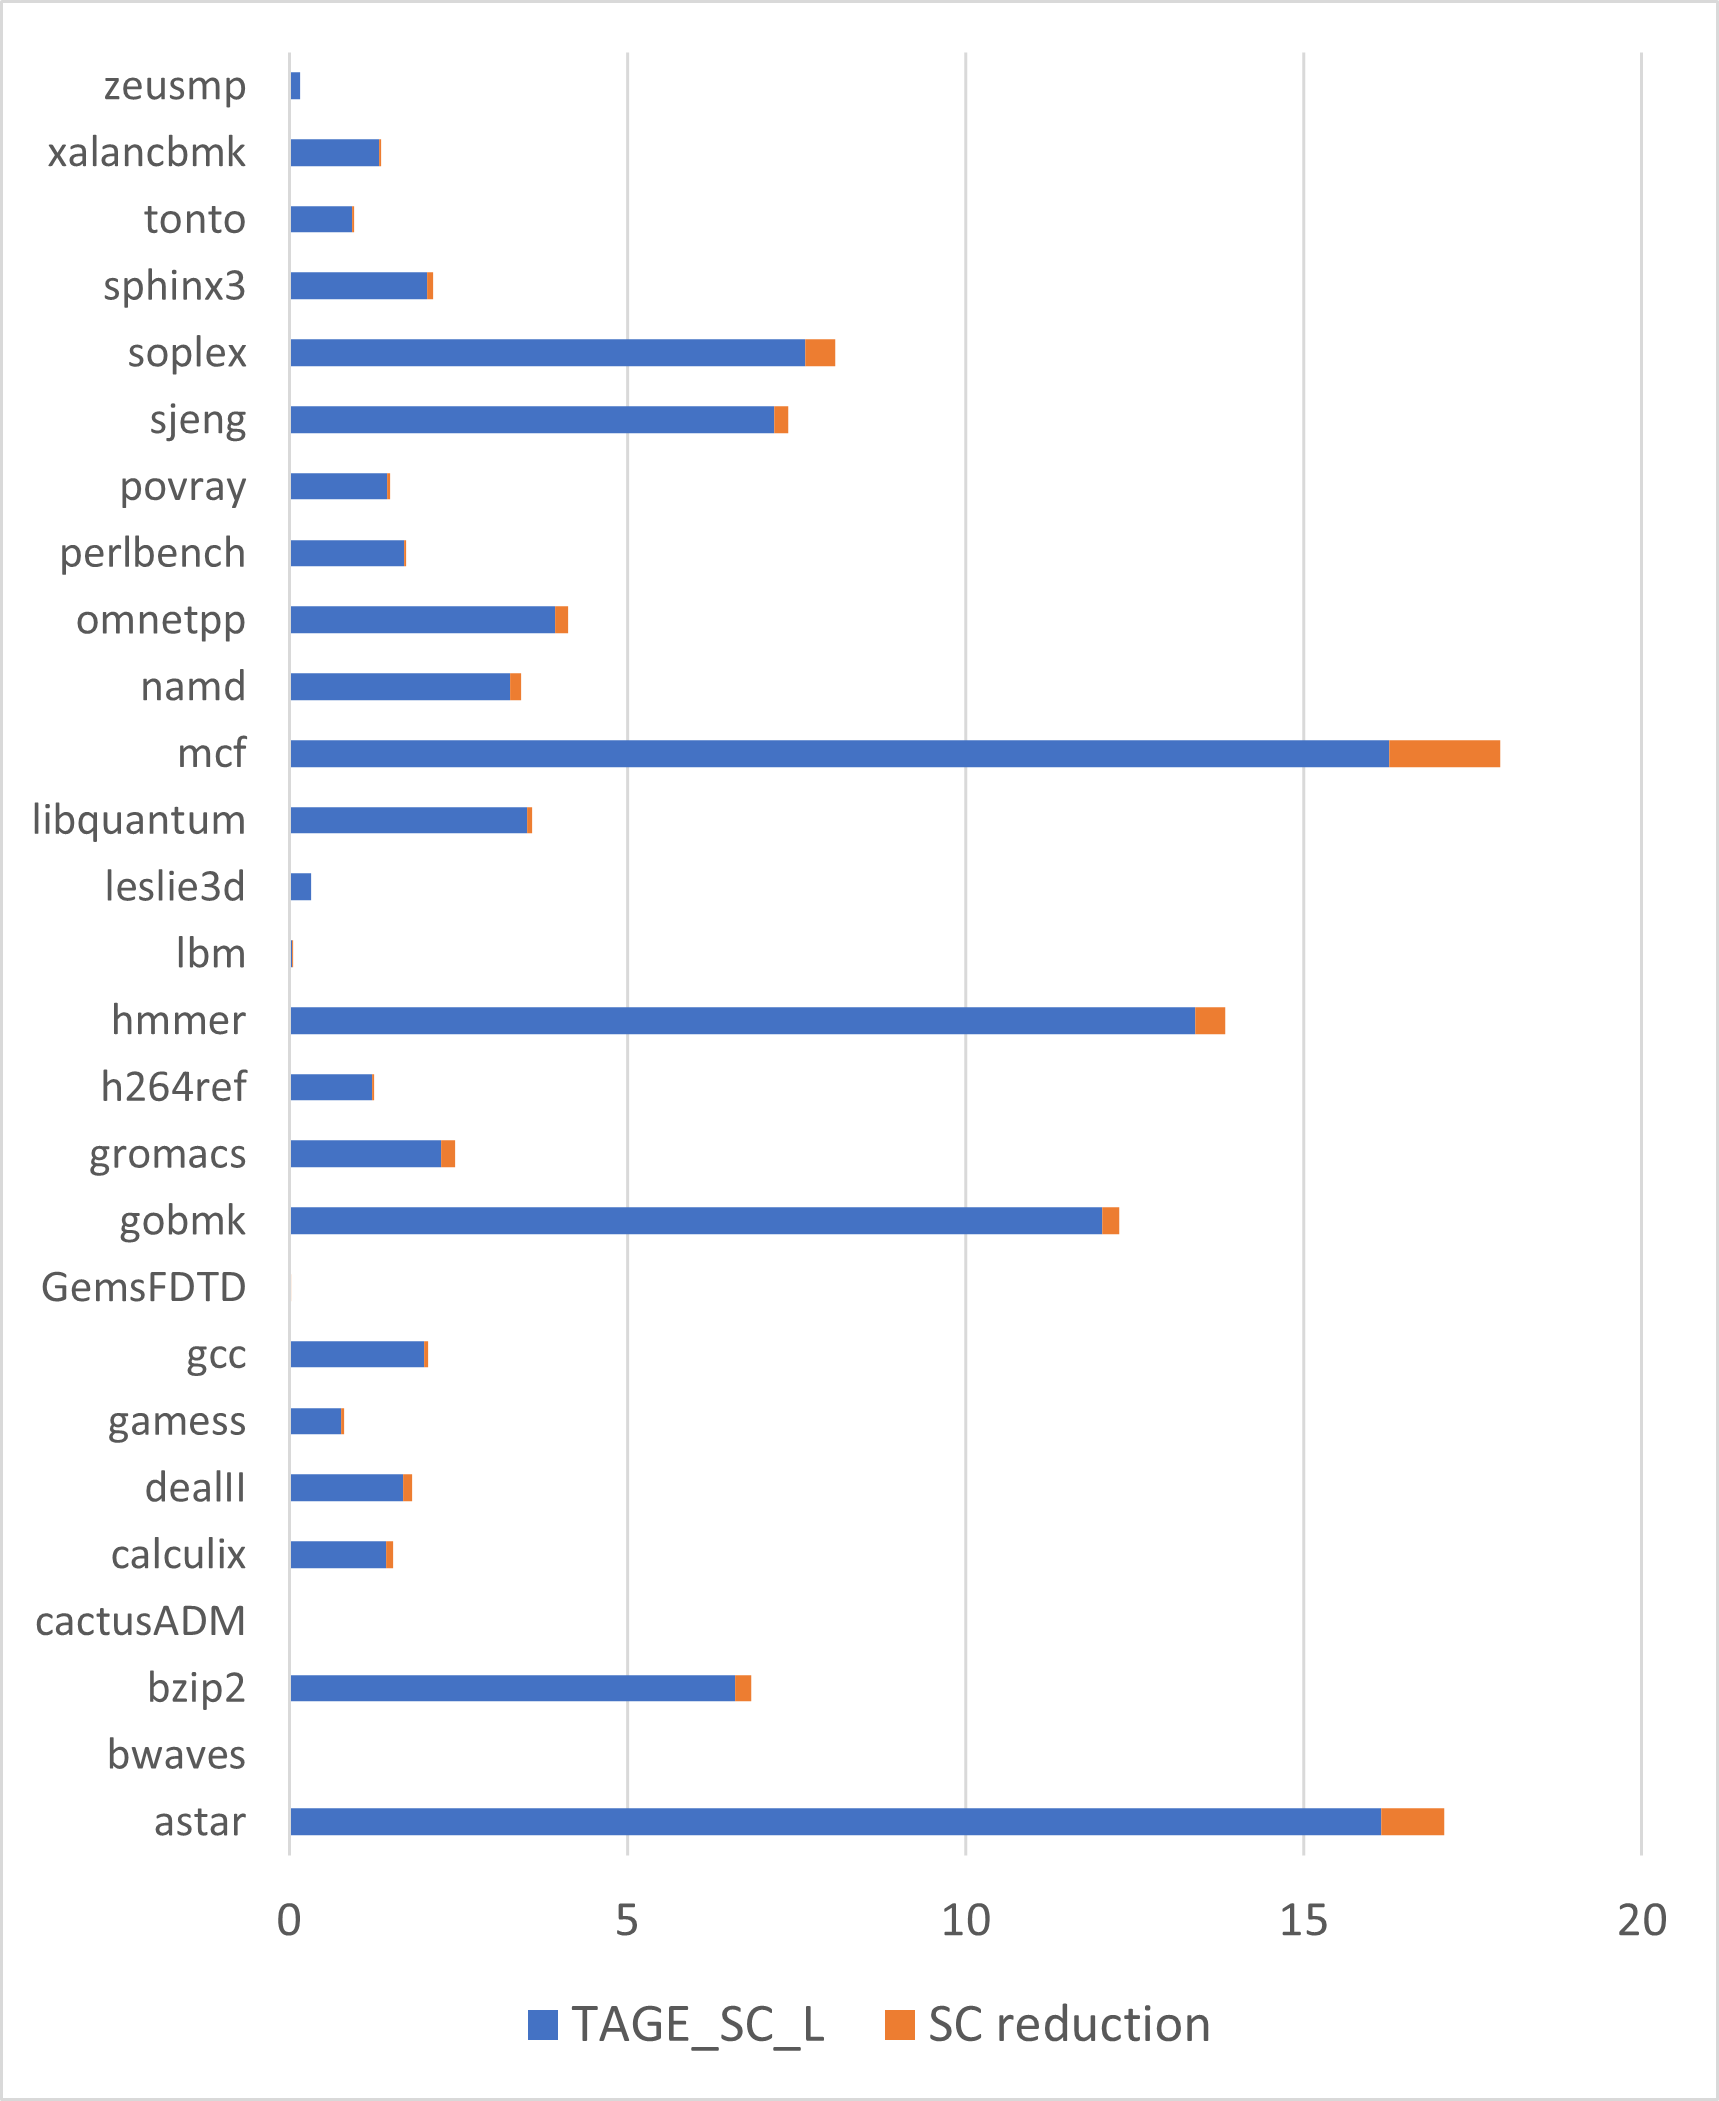
\includegraphics[width=\linewidth]{sc-mpki}
        \caption{SC降低的MPKI绝对值}
        \label{fig:sc-mpki}
    \end{subfigure}
    \begin{subfigure}{.45\textwidth}
        \centering
        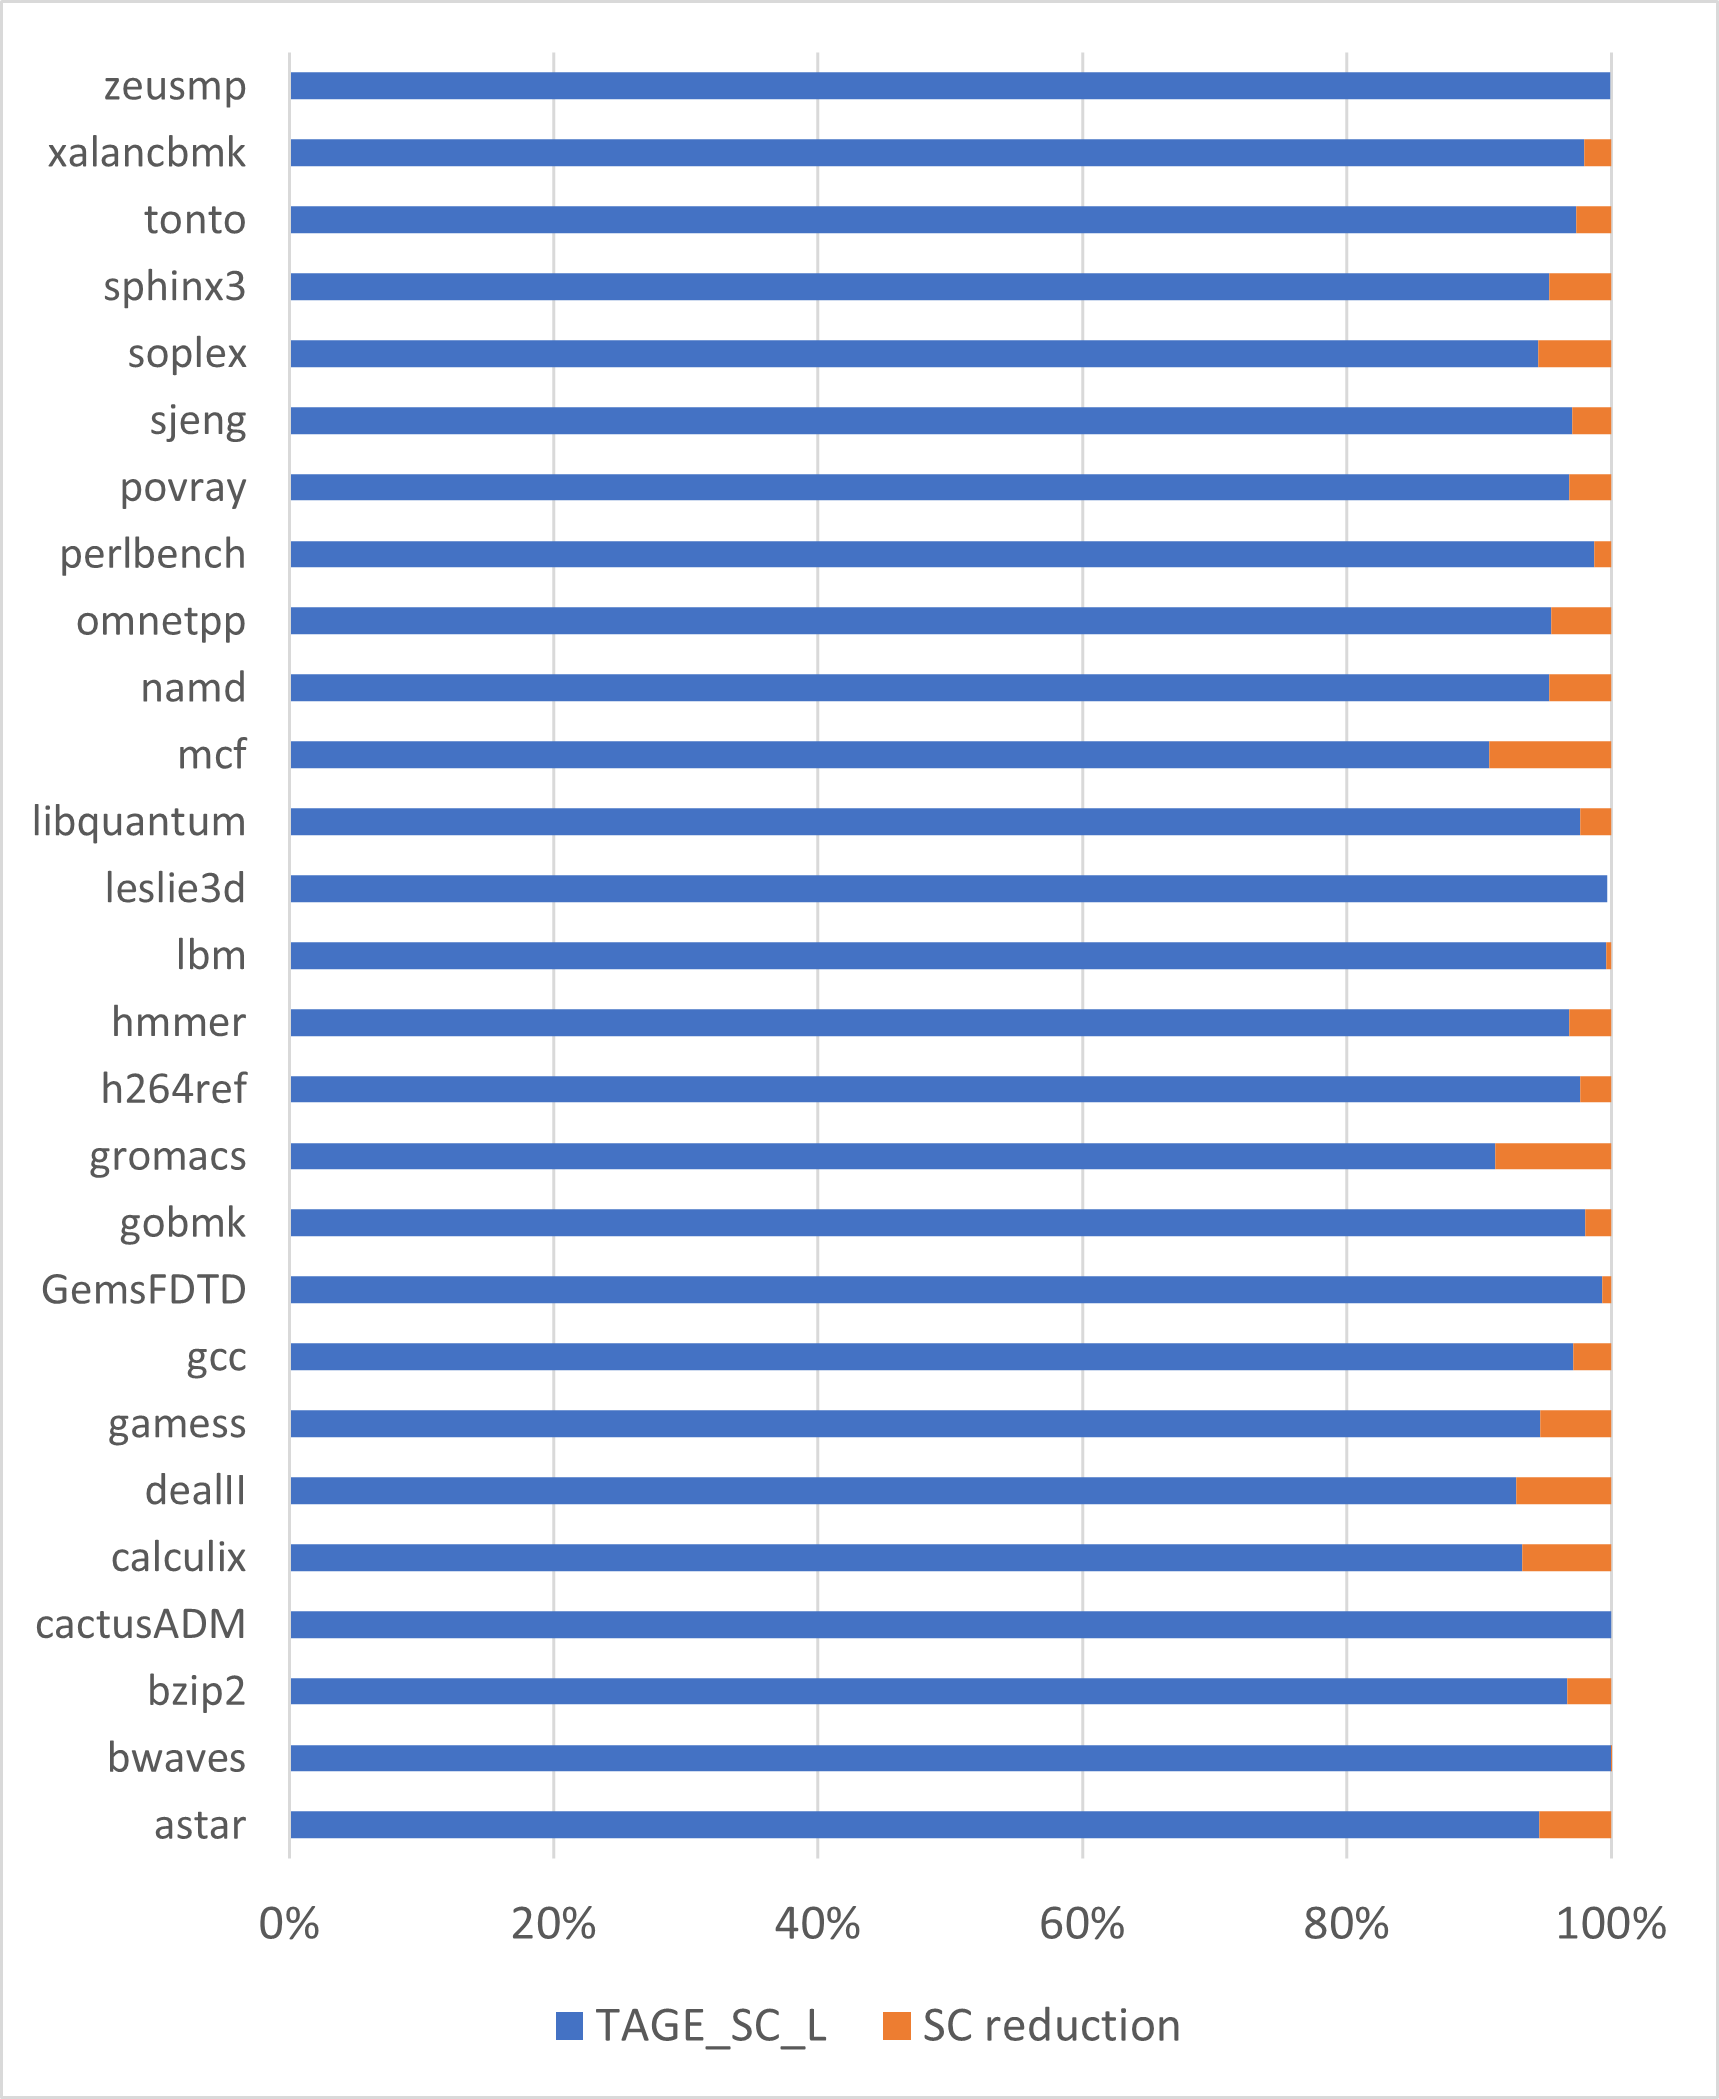
\includegraphics[width=\linewidth]{sc-mpki-rate}
        \caption{SC降低的MPKI百分比}
        \label{fig:sc-mpki-rate}
    \end{subfigure}
    \caption{Statistical Corrector对MPKI的降低}
    \label{fig:sc}
\end{figure}
我们在BOOM实现的LTAGE基础上,添加了Statistical Corrector实现。这个部件会检测某些LTAGE大概率预测错的情况进行修正,从而提升总体预测准确率。测试结果如图\ref{fig:sc},图\ref{fig:sc-mpki}中的蓝色柱形表示TAGE-SC-L的最终MPKI,橙色柱形表示在没有Statiscal Corrector的情况下会增加的MPKI;图\ref{fig:sc-mpki-rate}将图\ref{fig:sc-mpki}用百分比的形式呈现。在我们的测试集上,Statistical Corrector平均可以降低3\%左右的MPKI,可以看出该实现是有效果的。

\subsubsection*{三级预测各自对分支指令的预测准确率比较}
\begin{figure}[!htbp]
    \centering
    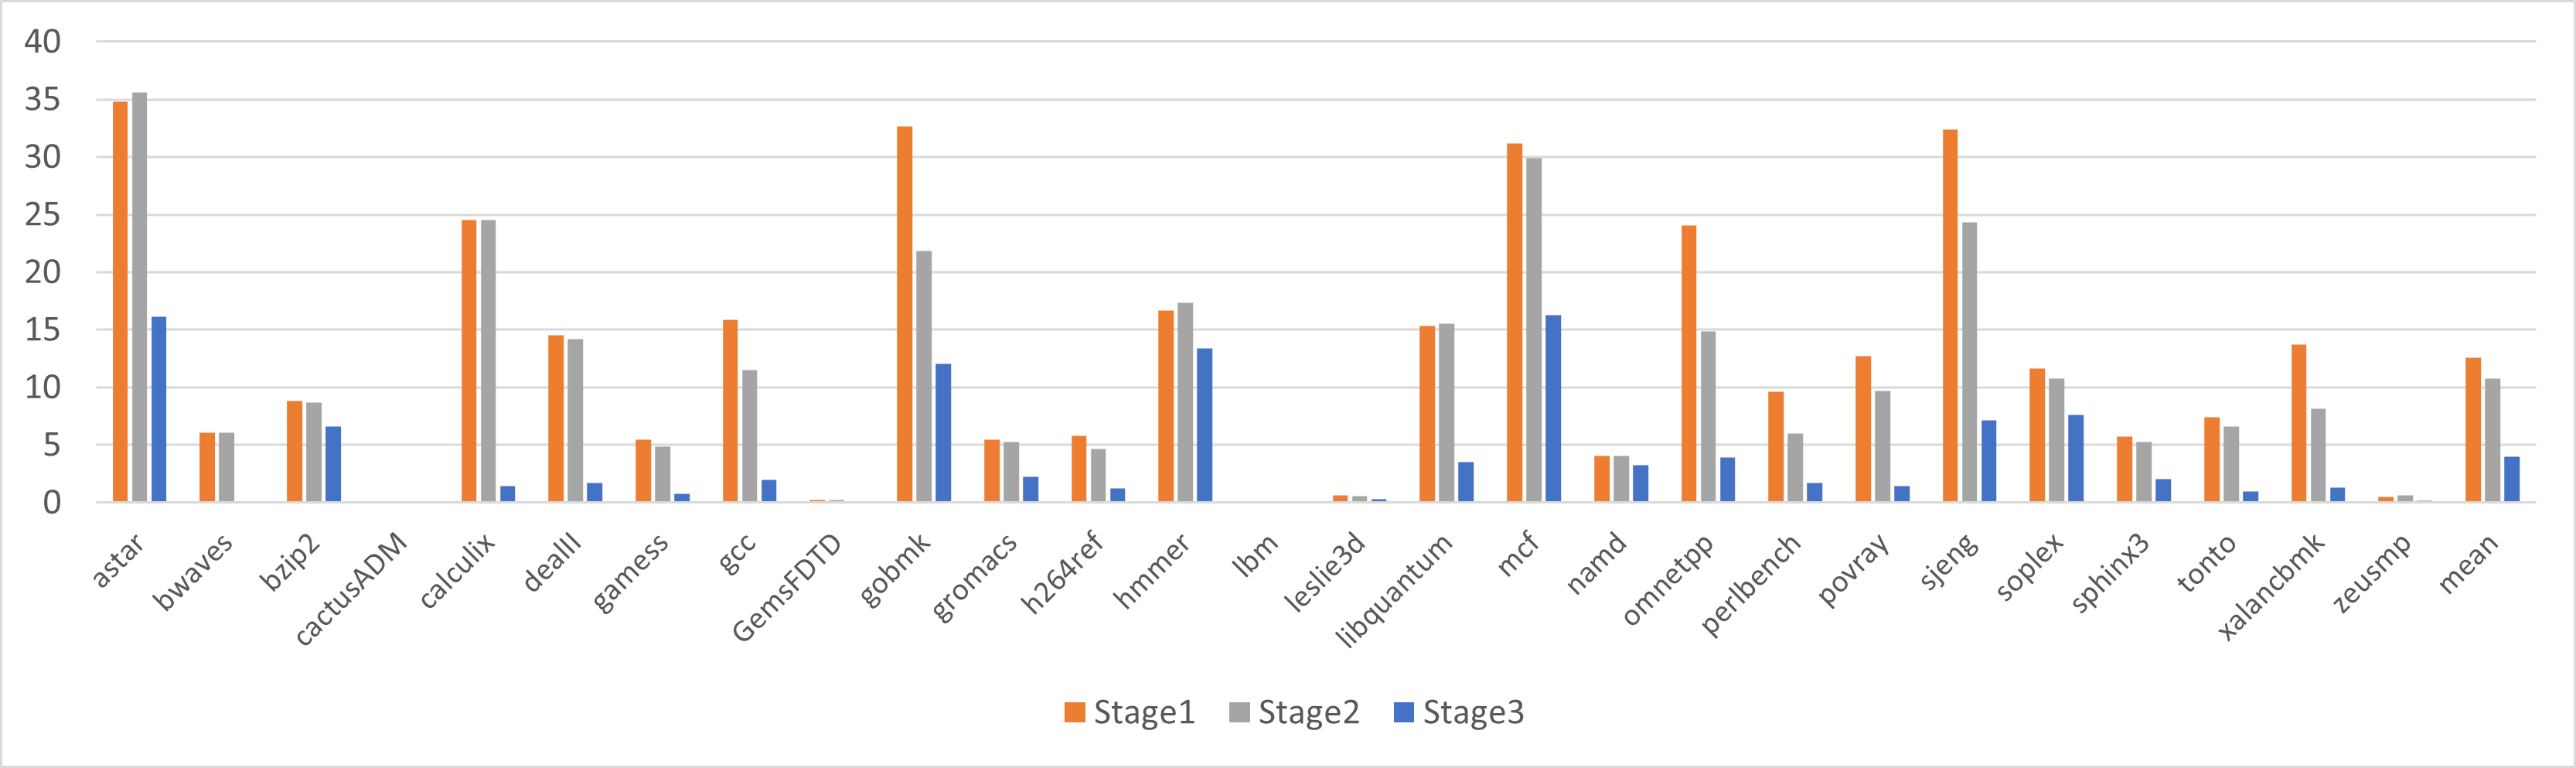
\includegraphics[width=\textwidth]{overriding-mpki}
    \caption{香山处理器分支预测各流水级的MPKI对比}
    \label{fig:overriding-mpki}
\end{figure}
\begin{table}[!htbp]
    \centering
    \footnotesize% fontsize
    \setlength{\tabcolsep}{4pt}% column separation
    \renewcommand{\arraystretch}{1.2}%row space 
    \begin{tabular}{cccc}
        %\cline{2-9}% partial hline from column i to column j
        \hline
        预测流水级 & Stage1 & Stage2 & Stage3 \\
        \hline
        MPKI      & 12.73  & 10.98  & 3.90 \\
        \hline
    \end{tabular}
    \caption{各级分支预测MPKI}
    \label{tab:overriding}
\end{table}
三级覆盖预测的假设中,后面流水级的预测一定比前面的流水级准,所以可以用后面的预测覆盖前面的预测。相邻两级的误预测率差距越大,后一级带来的性能收益越大。我们对各级的分支误预测情况进行了分别统计,得到数据如图\ref{fig:overriding-mpki}和表\ref{tab:overriding}。图\ref{fig:overriding-mpki}中“mean”的那一列表示所有测试项的平均值。可以看到,这些测试项之中主要存在几类情况:
\begin{enumerate}
    \item[\textbf{情况1}] 第一、二级MPKI差距不大,第三级MPKI显著低于其它两级,例如astar、mcf等;\label{overriding:cond1}
    \item[\textbf{情况2}] 第一、二级MPKI差距不大,第三级MPKI略低于其它两级,例如hmmer,bzip2等;\label{overriding:cond2}
    \item[\textbf{情况3}] 相邻流水级MPKI差距均相对较大,三级MPKI呈阶梯状分布,例如gobmk,omnetpp等;\label{overriding:cond3}
\end{enumerate}

第一级的条件分支预测依靠MicroBTB和两位饱和计数器;第二级的条件分支预测依靠BTB和两位饱和计数器。两级的预测机制并没有本质差别,区别仅在于使用的表项数目的多少。第一级可以预测最多256个目标地址和分支方向;第二级可以预测2048个目标地址和4096个分支方向。如果两级之间的预测差距不大,表明该测试的静态分支指令数目不多,且映射冲突不多;反之,则意味着测试中有很多静态指令或有着较多的映射冲突。情况1和情况2均属于前者。在全部的28个测试子项中,有21个子项有着这样的特性。因此第二级预测,目前在分支预测部件中起到的性能收益是相对较小的。后续可以在该级引入一个预测延迟为两拍的分支方向预测器,以提升该流水级对分支指令的预测性能。

图中还存在个别测试项中第二级误预测率略大于第一级的情况,例如astar和hmmer,这和我们的预期不符。如果实现符合设计的话,可能的原因是因为BTB存储的低位位数小于MicroBTB。出于时序考虑,我们在MicroBTB和BTB中仅存储分支指令目标地址的低位,在预测时用PC的高位与读出的低位拼接得到目标地址。在目标地址的高位和分支指令的PC不同时,会发生地址预测错误。MicroBTB存储了20位目标地址低位,而BTB只存储了13位目标地址低位。在RISC-V指令集中,分支指令的目标地址用该指令的PC与13位有符号偏移相加得到。对于目标地址的某一位来说,高位与原指令PC对应位不同的概率永远低于低位。这意味着,存储更少位地址的BTB在预测时更容易预测错目标地址。BTB的项数较多,存储开销已经较大,如果要存储更多的地址位数,会导致面积进一步增大。因此该问题的解决还需要进行进一步的考虑和评估。

最后一级预测有着最强的分支方向预测器,和预译码带来的准确的分支目标地址,因此带来了显著更低的MPKI。该级预测在多级覆盖预测的语境下是符合设计初衷的。

后续可以对前两级误预测做进一步的分类,区分误预测的原因究竟是因为方向预测错误还是目标地址缺失,从而指导进一步的优化。
\chapter{结论和展望}\label{chap:result}
本工作的目的是设计实现一款高性能的分支预测部件,满足香山RISC-V高性能处理器核的指令供给,以进一步支持香山处理器的流片。本工作在设计实现上进行了一些优化,在频率和性能方面都有提升。在主预测器上将SonicBOOM\cite{zhao2020sonicboom}分支预测部件中的L-TAGE预测器\cite{seznec2011new}进一步用Statistical Corrector\cite{seznec2014tage}加强。我们在仿真器和模拟器上进行性能对比评估表明,本工作的实现基本符合设计预期。后端评估结果表明,本工作在TSMC 28nm工艺下,频率能达到1.5GHz,相对SonicBOOM同规格配置下的分支预测器频率近乎提升一倍。

本工作实现的分支预测部件将随香山高性能处理器发布,源码也将一并开源,推动整个开源芯片领域的发展。

未来的工作可以从如下方向进行:
\begin{enumerate}
    \item 目前的工作中尚未包括间接跳转预测器的实现,而现代程序设计语言中例如虚函数表的实现会在程序中大量引入间接跳转指令。一个完善的间接跳转预测器将会在这方面减少大量的误预测,提升处理器的整体性能;
    \item 目前实现的主分支预测器是原设计的一种简化实现,具体表现在如下方面:
    \begin{itemize}
        \item 所使用的分支历史长度较短,历史表不多;
        \item 未实现Immediate Update Mimicker\cite{seznec2011new}
    \end{itemize}
    针对上述两个方面进行进一步优化后,预计分支误预测率可以进一步降低;
    \item 目前的时序只能满足1.5GHz,高性能设计要求更高的主频,因此需要对时序进行进一步优化。
\end{enumerate}
%---------------------------------------------------------------------------%
% main content
%-
%-> Appendix
%-
% \cleardoublepage%
% \appendix% initialize the environment
% \chapter{分支预测背景知识}\label{appendix:background}
本章节简要介绍本设计中用到的分支预测部件的背景知识。
\section{TAGE分支方向预测器}
TAGE分支方向预测器的主要任务有三项:预测、更新和回滚。作为通过历史信息决定预测结果的部件,它的主要存储开销用来维护M+1张记录历史分支信息的表。其中有一张表是一个直接用分支指令地址索引的bimodal基预测器,而另外M张表分别使用不同长度的分支历史和分支地址进行哈希索引,这些分支历史的长度依次形成几何级数。每一张表采用了类似cache的带标签的存储方式,用前述的哈希值查找得到一个表项后,将其中的tag与PC和分支历史的另一种哈希值进行匹配。在预测时,所有的表会进行并行查找,仅当某张表的tag匹配成功时,它才能提供候选预测值。最终的预测结果由能提供预测结果的使用最长历史信息的表提供。如果M张表的标签都匹配失败,那么使用bimodal基预测器的预测结果。下图为M=4的TAGE分支预测器结构示例,其中bimodal表项均为两位饱和计数器,而M张带标签的表的表项由三部分组成:pred、tag、u。其中pred为提供预测结果的三位饱和计数器,它的最高有效位决定了预测方向;tag为10~13位标签;u是useful counter的简称,它是一个两位饱和计数器,会影响TAGE更新时的行为。

TAGE的更新机制是它的关键所在。将此次预测中决定最终结果的表记为provider,provider即为当次预测中标签匹配成功且使用了最长历史的表。将标签匹配成功且使用次长历史的表记为altpred。

Pred域的更新:若预测结果正确,则依预测结果更新provider中对应表项中的pred域;反之,除了以相同方法更新provider的pred域以外,假如provider并不是所有表中使用最长历史的那张表,则试图在更长历史的那些表中选择一张表分配一个表项给这条分支。具体的分配策略决定于这些表中对应表项	useful counter的值:如果所有对应表项的useful counter都大于0,则将它们都减一,此次不分配新的表项;如果存在某个u=0的表项,则它可以被分配给这条分支;如果存在至少两个u=0的表项,则以更倾向于历史长度较低表项的概率分配表项(进一步阐述)。分配后表项pred域初始化为weak correct(例如0),u域初始化为0。

Useful域的更新:当altpred的结果与provider不同时,更新provider的u域。此时如果provider的结果正确,u增1,反之u减1。Useful域实行定期flush机制,每隔256K条分支,将一排u域的MSB清零。

某次分支预测的回滚需要保存做出预测前一刻预测器内的一些信息,以及该次预测中产生的某些信息。这些信息打包后送入BRQ,以待用于回滚和更新。% appendix content
%-
%-> Backmatter: bibliography, glossary, index
%-
\backmatter% initialize the environment
\intotoc*{\cleardoublepage}{\bibname}% add link to toc
\artxifstreq{\artxbib}{bibtex}{% enable bibtex
    \bibliography{Biblio/ref}% bibliography
}{%
    \printbibliography% bibliography
}
%---------------------------------------------------------------------------%
%->> Backmatter
%---------------------------------------------------------------------------%
\chapter{作者简历}
\noindent
姓名:勾凌睿\quad\quad 性别:男\quad\quad 出生日期:1998.8.31\quad\quad 籍贯:黑龙江
\noindent
\begin{flalign*}
    &2015.9 -- 2019.6       &\mbox{中国科学院大学计算机科学技术专业本科生}\\
    &2019.9 -- \mbox{现在}  &\mbox{中国科学院计算技术研究所硕士研究生}
\end{flalign*}


\section*{【攻读硕士学位期间发表的论文】}
无

\section*{【攻读硕士学位期间参加的科研项目】}
香山RISC-V高性能处理器核开发

\section*{【攻读硕士学位期间的获奖情况】}
无

{
\setlist[enumerate]{}% restore default behavior
% \begin{enumerate}[nosep]
%     \item ucasthesis: A LaTeX Thesis Template for the University of Chinese Academy of Sciences, 2014.
% \end{enumerate}
}

\chapter[致谢]{致\quad 谢}\chaptermark{致\quad 谢}% syntax: \chapter[目录]{标题}\chaptermark{页眉}
\thispagestyle{noheaderstyle}% 如果需要移除当前页的页眉
%\pagestyle{noheaderstyle}% 如果需要移除整章的页眉
感谢我的指导老师包云岗研究员为我提供的研究机会和悉心指导。

感谢项目组的唐老师、郇老师、赵老师、李老师在本工作过程中提供的宝贵经验和方向指导。

感谢本组的师兄师姐、同学和师弟师妹们,在大家的通力协作下,项目取得了很大的进展。

感谢父母一路上的支持和关心,你们给了我力量,让我有能力在更大的平台上施展拳脚。
\cleardoublepage[plain]% 让文档总是结束于偶数页,可根据需要设定页眉页脚样式,如 [noheaderstyle]
%---------------------------------------------------------------------------%
% other information
\end{document}
%---------------------------------------------------------------------------%

